\documentclass[12pt,a4paper]{article}

\usepackage[utf8]{inputenc}
\usepackage[T1]{fontenc}
\usepackage{lmodern}
\usepackage{textcomp}
\usepackage{newunicodechar}
\usepackage[margin=2.5cm]{geometry}
\usepackage{amsmath,amssymb}
\usepackage{graphicx}
\usepackage{listings}
\usepackage{xcolor}
\usepackage{hyperref}
\usepackage{fancyhdr}
\usepackage{float}
\usepackage{booktabs}
\usepackage{caption}
\usepackage{tabularx}
\usepackage{array}
\usepackage{tikz}
\usetikzlibrary{trees,positioning,shapes.geometric}

% Adjust header height for fancyhdr
\setlength{\headheight}{15pt}
\addtolength{\topmargin}{-3pt}

% Romanian Unicode support for standard pdflatex
\newunicodechar{Ă}{\v{A}}
\newunicodechar{ă}{\v{a}}
\newunicodechar{Â}{\^{A}}
\newunicodechar{â}{\^{a}}
\newunicodechar{Î}{\^{I}}
\newunicodechar{î}{\^{i}}
\newunicodechar{Ș}{\c{S}}
\newunicodechar{ș}{\c{s}}
\newunicodechar{Ț}{\c{T}}
\newunicodechar{ț}{\c{t}}

\hypersetup{
    colorlinks=true,
    linkcolor=blue,
    filecolor=magenta,      
    urlcolor=cyan,
    citecolor=blue
}

% Colors for code listings
\definecolor{codebg}{gray}{0.96}
\definecolor{codegreen}{rgb}{0.13,0.55,0.13}
\definecolor{codegray}{rgb}{0.5,0.5,0.5}
\definecolor{codepurple}{rgb}{0.58,0,0.82}
\definecolor{codeblue}{rgb}{0.05,0.25,0.70}

\lstset{
    backgroundcolor=\color{codebg},
    basicstyle=\ttfamily\footnotesize,
    breaklines=true,
    breakatwhitespace=true,
    frame=single,
    rulecolor=\color{gray!40},
    keepspaces=true,
    showstringspaces=false,
    upquote=true,
    columns=fullflexible,
    tabsize=2
}

\lstdefinestyle{cstyle}{
    language=C,
    commentstyle=\color{codegreen}\itshape,
    keywordstyle=\color{codeblue}\bfseries,
    stringstyle=\color{codepurple},
    numbers=left,
    numbersep=7pt,
    numberstyle=\tiny\color{codegray},
    stepnumber=1
}

\lstdefinestyle{bashstyle}{
    language=bash,
    commentstyle=\color{codegreen}\itshape,
    keywordstyle=\color{codeblue}\bfseries,
    stringstyle=\color{codepurple},
    numbers=left,
    numbersep=7pt,
    numberstyle=\tiny\color{codegray},
    stepnumber=1
}

\lstdefinestyle{consolestyle}{
    backgroundcolor=\color{codebg},
    basicstyle=\ttfamily\footnotesize,
    breaklines=true,
    frame=single,
    rulecolor=\color{gray!40},
    numbers=none
}

% Header and Footer
\pagestyle{fancy}
\fancyhf{}
\lhead{Operating Systems -- Lab 7}
\rhead{Iulian Pavlov, FAF-241}
\cfoot{\thepage}

\begin{document}

% ============================================================================
% TITLE PAGE
% ============================================================================
\begin{titlepage}
\begin{center}
    
\includegraphics[width=0.3\textwidth]{logo.png} \\[0.2cm] 
    
    \textbf{MINISTRY OF EDUCATION, CULTURE AND RESEARCH \\ OF THE REPUBLIC OF MOLDOVA} \\[0.3cm]
    
    \textbf{Technical University of Moldova \\ Faculty of Computers, Informatics and Microelectronics \\ Department of Software and Automation Engineering} \\[1.8cm]
    
    \textbf{Iulian Pavlov, FAF-241}\\[0.5cm]
    
    \Huge \textbf{Report} \\[0.5cm]
    
    \large Laboratory work nr. 7 \\[0.5cm]
    
    \textbf{\Large Processes, Signals, and Pipelines} \\[0.3cm]
    \normalsize Course: Operating Systems (Track A: Linux) \\[2.2cm]

    \begin{flushright}
        \textit{Checked by:} \\
        \textbf{Reițman Patricia}, \textit{University Assistant} \\
        Department of Software and Automation Engineering, \\
        FCIM Faculty, UTM 
    \end{flushright}
    \vfill
    
    Chișinău -- 2026
\end{center}
\end{titlepage}

\pagenumbering{roman}
\newpage
\tableofcontents
\newpage
\pagenumbering{arabic}

% ============================================================================
% 1. THEORETICAL BACKGROUND & OBJECTIVES
% ============================================================================
\section{Theoretical Background and Objectives}

\subsection{Laboratory Objectives and Scope}
In UNIX and modern Linux operating systems, the process abstraction is the primary mechanism for computational isolation and concurrency. The primary objective of Laboratory Work Nr.~7 is to explore the Linux process model, process execution lifecycle, standard stream redirection, and inter-process communication (IPC) via pipes.

Throughout this laboratory, we investigate:
\begin{itemize}
    \item \textbf{Tracing Process Management Syscalls (\texttt{strace})}: Observing how the shell orchestrates pipelines via anonymous pipes (\texttt{pipe2}), process replication (\texttt{clone}), file descriptor reassignment (\texttt{dup2}), and executable loading (\texttt{execve}).
    \item \textbf{Process Lifecycle, Concurrency, and Reaping}: Utilizing \texttt{fork()} and \texttt{waitpid()} to spawn concurrent child processes, monitor execution states, and harvest exit statuses using POSIX macros (\texttt{WIFEXITED}, \texttt{WEXITSTATUS}, \texttt{WIFSIGNALED}, \texttt{WTERMSIG}).
    \item \textbf{Zombie and Orphan Management}: Observing zombie processes in state \texttt{Z} (\texttt{<defunct>}) using \texttt{ps}, examining the responsibilities of parent processes in status harvesting, and understanding reparenting to PID 1.
    \item \textbf{Exponential Process Trees}: Analyzing process duplication across sequential \texttt{fork()} invocations and verifying the resulting $2^n$ process tree topology.
    \item \textbf{I/O Buffering and Address Space Duplication}: Analyzing the critical difference between line-buffered interactive terminals (TTY) and block-buffered pipes/files, explaining duplicate prints from un-flushed libc buffers across \texttt{fork()}.
    \item \textbf{Program Execution and Signal Trapping (\texttt{myrun})}: Building a wrapper utility around \texttt{execvp} to execute binaries, pass arguments, handle execution failures, and detect termination by asynchronous signals (e.g., \texttt{SIGTERM}).
    \item \textbf{Stream Redirection (\texttt{redirect} and \texttt{myrun2})}: Manipulating per-process open file descriptor tables using \texttt{dup2()} to route standard output (\texttt{STDOUT\_FILENO}) to regular filesystem files.
    \item \textbf{Inter-Process Communication Pipelines (\texttt{pipeline} and \texttt{pipeline3})}: Developing two-stage and three-stage data processing pipelines using anonymous pipes, coordinating data flow between stages, and avoiding deadlocks through disciplined file descriptor closing.
\end{itemize}

\subsection{Core Systems Architecture Concepts}
\begin{enumerate}
    \item \textbf{The Fork-Exec-Wait Paradigm}: Unlike operating systems that spawn processes via a single unified call (such as \texttt{CreateProcess} on Windows), UNIX decouples process creation from executable loading. \texttt{fork()} duplicates the calling process's entire virtual address space, memory pages (via Copy-On-Write), and file descriptor table. The child process can subsequently modify its environment and descriptor table before calling \texttt{execve()}, which replaces the process memory image with a new binary.
    \item \textbf{File Descriptors and the Open File Table}: Every process has a file descriptor table. Standard slots 0, 1, and 2 correspond to \texttt{stdin}, \texttt{stdout}, and \texttt{stderr}. The system call \texttt{dup2(oldfd, newfd)} atomically closes \texttt{newfd} (if open) and duplicates \texttt{oldfd} into slot \texttt{newfd}, sharing the underlying open file description and file offset pointer.
    \item \textbf{Anonymous Pipes}: An anonymous pipe is a unidirectional FIFO byte stream allocated in kernel memory with a designated read end (\texttt{p[0]}) and write end (\texttt{p[1]}). Readers block when data is temporarily unavailable. Crucially, a reader receives \texttt{EOF} (0 bytes read) if and only if \textbf{every} open file descriptor pointing to the write end of the pipe across all processes in the system has been closed.
\end{enumerate}

\newpage

% ============================================================================
% 2. PART 1: TRACING EXECUTION MECHANICS WITH STRACE
% ============================================================================
\section{Part 1: Tracing Execution Mechanics with \texttt{strace}}

\subsection{Tracing a Pipelined Command}
We ran \texttt{strace} with the \texttt{-f} flag (to follow child processes) and filtered for process management and I/O syscalls while executing the pipeline \texttt{ls / | wc -l} in GNU Bash:

\begin{lstlisting}[style=consolestyle]
$ strace -f -e trace=pipe2,clone,clone3,dup2,execve,wait4 bash -c 'ls / | wc -l'
execve("/usr/bin/bash", ["bash", "-c", "ls / | wc -l"], 0x7ffd1ada4d18 /* 199 vars */) = 0
pipe2([3, 4], 0)                        = 0
clone(child_stack=NULL, flags=CLONE_CHILD_CLEARTID|CLONE_CHILD_SETTID|SIGCHLD, child_tidptr=0x7eb6a3a42e50) = 15021
strace: Process 15021 attached
[pid 15020] clone(child_stack=NULL, flags=CLONE_CHILD_CLEARTID|CLONE_CHILD_SETTID|SIGCHLD, child_tidptr=0x7eb6a3a42e50) = 15022
[pid 15021] dup2(4, 1)                  = 1
strace: Process 15022 attached
[pid 15020] wait4(-1 <unfinished ...>
[pid 15022] dup2(3, 0)                  = 0
[pid 15021] execve("/usr/bin/ls", ["ls", "/"], 0x5bf3950f21b0 /* 199 vars */ <unfinished ...>
[pid 15022] execve("/usr/bin/wc", ["wc", "-l"], 0x5bf3950f21b0 /* 199 vars */ <unfinished ...>
[pid 15021] <... execve resumed>)       = 0
[pid 15021] +++ exited with 0 +++
[pid 15020] <... wait4 resumed>, [{WIFEXITED(s) && WEXITSTATUS(s) == 0}], 0, NULL) = 15021
[pid 15020] wait4(-1 <unfinished ...>
[pid 15022] <... execve resumed>)       = 0
19
[pid 15022] +++ exited with 0 +++
<... wait4 resumed>, [{WIFEXITED(s) && WEXITSTATUS(s) == 0}], 0, NULL) = 15022
--- SIGCHLD {si_signo=SIGCHLD, si_code=CLD_EXITED, si_pid=15021, si_uid=1000, si_status=0, si_utime=0, si_stime=0} ---
wait4(-1, 0x7ffeff115694, WNOHANG, NULL) = -1 ECHILD (No child processes)
+++ exited with 0 +++
\end{lstlisting}

\subsection{System Call Profiling of \texttt{ls}}
We profiled the system calls issued by \texttt{ls} when reading the directory \texttt{/usr/bin}:

\begin{lstlisting}[style=consolestyle]
$ strace -c ls /usr/bin > /dev/null
% time     seconds  usecs/call     calls    errors syscall
------ ----------- ----------- --------- --------- ----------------
 56.20    0.000843         140         6           getdents64
 25.73    0.000386         386         1           execve
  7.67    0.000115           8        14           mmap
  2.60    0.000039           9         4           mremap
  1.53    0.000023           4         5           openat
  1.47    0.000022           3         6           brk
  1.27    0.000019           6         3           newfstatat
  1.13    0.000017           2         6           fstat
  0.73    0.000011           1         7           close
  0.67    0.000010           0        12           write
  0.60    0.000009           4         2           read
  0.33    0.000005           5         1         1 access
  0.07    0.000001           0         2         2 ioctl
------ ----------- ----------- --------- --------- ----------------
100.00    0.001500          17        87         7 total
\end{lstlisting}

\subsection{Answers to Questions (Part 1)}

\subsubsection*{(1) In what order do \texttt{pipe2}, \texttt{clone}, \texttt{dup2} and \texttt{execve} appear? Which process (PID) calls \texttt{dup2(.., 1)} and which calls \texttt{dup2(.., 0)}? Explain why in one sentence each.}
\begin{itemize}
    \item \textbf{Syscall Order}: 
    \begin{align*}
        \texttt{pipe2} &\;\longrightarrow\; \texttt{clone}\text{ (child 1)} \;\longrightarrow\; \texttt{clone}\text{ (child 2)} \\
        &\;\longrightarrow\; \texttt{dup2}\text{ (in each child)} \;\longrightarrow\; \texttt{execve}\text{ (in each child)}
    \end{align*}
    The parent bash process first creates the communication channel with \texttt{pipe2([3, 4], 0)}, then clones both child processes, after which each child binds its standard streams via \texttt{dup2} before finally executing its respective binary via \texttt{execve}.
    \item \textbf{\texttt{dup2(4, 1)} Caller}: Process \textbf{PID 15021} (\texttt{ls}) calls \texttt{dup2(4, 1)} to bind its standard output (\texttt{fd 1}) to the write end of the pipe (\texttt{fd 4}) so that directory listing data is piped forward.
    \item \textbf{\texttt{dup2(3, 0)} Caller}: Process \textbf{PID 15022} (\texttt{wc}) calls \texttt{dup2(3, 0)} to bind its standard input (\texttt{fd 0}) to the read end of the pipe (\texttt{fd 3}) so that line counting consumes the data streamed through the pipe.
\end{itemize}

\subsubsection*{(2) On Linux there is no "fork" line. Which call creates the children instead?}
On Linux, the \textbf{\texttt{clone}} (or \textbf{\texttt{clone3}}) system call creates the child processes instead of a traditional \texttt{fork} syscall. In the GNU C Library (glibc), \texttt{fork()} is implemented as a specialized invocation of:
\begin{center}
\texttt{clone(child\_stack=NULL, flags=CLONE\_CHILD\_CLEARTID | CLONE\_CHILD\_SETTID | SIGCHLD, ...)}
\end{center}
The \texttt{clone} syscall offers a unified, extensible interface that underpins both process creation and POSIX thread instantiation (\texttt{pthreads}) by parametrically controlling which virtual memory, file descriptor tables, and namespaces are copied or shared.

\subsubsection*{(3) How many write calls does \texttt{ls} make to print all of \texttt{/usr/bin}? Why so few?}
\texttt{ls} issued only \textbf{12 \texttt{write} calls} to output several thousand binary names. This efficiency is achieved through \textbf{user-space stream buffering} implemented by the C standard library (\texttt{libc}). Rather than issuing an individual kernel-crossing \texttt{write()} system call for each individual file string, formatted output is accumulated inside an internal user-space buffer (typically 4096 or 8192 bytes) and flushed in large, contiguous blocks, minimizing context switches between user and kernel mode.

\newpage

% ============================================================================
% 3. PART 2: PROCESS CREATION, ZOMBIES, QUIZ, AND I/O BUFFERING
% ============================================================================
\section{Part 2: Process Creation, Zombies, Quiz, and I/O Buffering}

\subsection{Basic Fork and Status Retrieval (\texttt{fork.c})}
We created and compiled \texttt{fork.c} to inspect process IDs and exit status harvesting:

\begin{lstlisting}[style=cstyle]
#include <stdio.h>
#include <stdlib.h>
#include <unistd.h>
#include <sys/wait.h>

int main(void)
{
    printf("before fork: pid=%d\n", getpid());
    fflush(stdout);

    pid_t pid = fork();
    if (pid < 0) { 
        perror("fork"); 
        exit(1); 
    }

    if (pid == 0) { /* child */
        printf("child: pid=%d parent=%d\n", getpid(), getppid());
        exit(42);
    }

    int status; /* parent */
    waitpid(pid, &status, 0);
    printf("parent: pid=%d, my child %d exited with %d\n",
           getpid(), pid, WEXITSTATUS(status));
    return 0;
}
\end{lstlisting}

Execution trace:
\begin{lstlisting}[style=consolestyle]
$ gcc -Wall -Wextra -o fork fork.c && ./fork
before fork: pid=16968
child: pid=16969 parent=16968
parent: pid=16968, my child 16969 exited with 42
\end{lstlisting}

\subsection{Observing Zombie Processes (\texttt{zombie.c})}
To observe the zombie process state, we developed \texttt{zombie.c}, where the child terminates immediately while the parent sleeps without calling \texttt{wait()}:

\begin{lstlisting}[style=cstyle]
#include <stdio.h>
#include <stdlib.h>
#include <unistd.h>

int main(void)
{
    pid_t pid = fork();

    if (pid < 0) {
        perror("fork");
        exit(1);
    }

    if (pid == 0) {
        printf("Child (PID %d) is exiting now...\n", getpid());
        exit(0);
    } else {
        printf("Parent (PID %d) created child (PID %d).\n", getpid(), pid);
        printf("Parent sleeping for 30 seconds. Check `ps` in another terminal!\n");
        sleep(30);
        printf("Parent waking up and exiting.\n");
    }

    return 0;
}
\end{lstlisting}

We launched the program in the background and queried the process table:
\begin{lstlisting}[style=consolestyle]
$ gcc -Wall -Wextra -o zombie zombie.c
$ ./zombie &
[2] 17428
Parent (PID 17428) created child (PID 17430).
Parent sleeping for 30 seconds. Check `ps` in another terminal!
Child (PID 17430) is exiting now...

$ sleep 1; ps -o pid,ppid,stat,cmd --ppid $!
    PID    PPID STAT CMD
  17430   17428 Z    [zombie] <defunct>

Parent waking up and exiting.
\end{lstlisting}

\subsection{Process Tree Doubling Quiz (\texttt{quiz.c})}
We implemented \texttt{quiz.c} containing three consecutive \texttt{fork()} invocations:

\begin{lstlisting}[style=cstyle]
#include <stdio.h>
#include <unistd.h>

int main(void) {
    fork();
    fork();
    fork();
    printf("hi\n");
    return 0;
}
\end{lstlisting}

Execution and output line count:
\begin{lstlisting}[style=consolestyle]
$ gcc -Wall -o quiz quiz.c && ./quiz | wc -l
8
\end{lstlisting}

\begin{figure}[H]
\centering
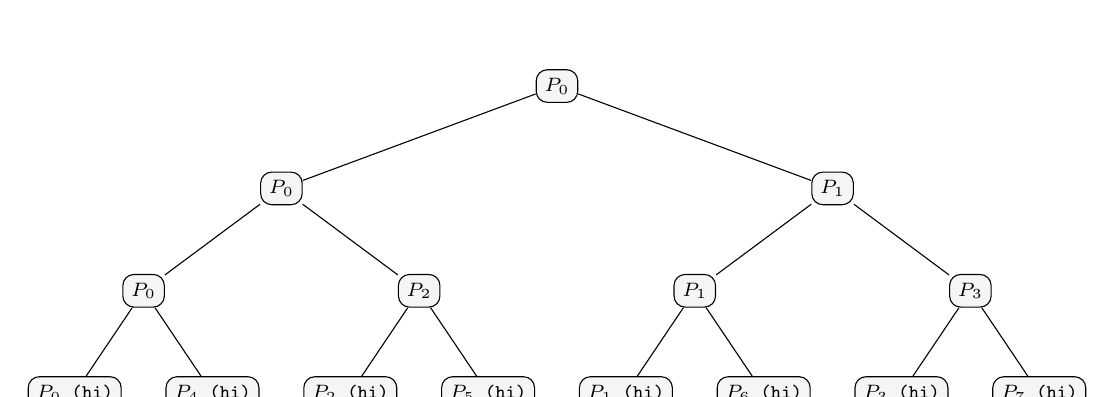
\begin{tikzpicture}[
    level 1/.style={sibling distance=7.0cm, level distance=1.3cm},
    level 2/.style={sibling distance=3.5cm, level distance=1.3cm},
    level 3/.style={sibling distance=1.75cm, level distance=1.3cm},
    every node/.style={rectangle, draw, rounded corners, fill=codebg, inner sep=3pt, font=\scriptsize\ttfamily}
]
\node {$P_0$}
    child { node {$P_0$}
        child { node {$P_0$}
            child { node {$P_0$ (hi)} }
            child { node {$P_4$ (hi)} }
        }
        child { node {$P_2$}
            child { node {$P_2$ (hi)} }
            child { node {$P_5$ (hi)} }
        }
    }
    child { node {$P_1$}
        child { node {$P_1$}
            child { node {$P_1$ (hi)} }
            child { node {$P_6$ (hi)} }
        }
        child { node {$P_3$}
            child { node {$P_3$ (hi)} }
            child { node {$P_7$ (hi)} }
        }
    };
\end{tikzpicture}
\caption{Process Tree generated by three successive \texttt{fork()} calls in \texttt{quiz.c} resulting in 8 distinct processes.}
\label{fig:processtree}
\end{figure}

\subsection{I/O Buffering Mechanics (\texttt{./fork} vs. \texttt{./fork | cat})}
When \texttt{fflush(stdout)} was commented out in \texttt{fork.c}, we observed differing behavior between terminal execution and pipe redirection:

\begin{lstlisting}[style=consolestyle]
$ ./fork
before fork: pid=18134
child: pid=18135 parent=18134
parent: pid=18134, my child 18135 exited with 42

$ ./fork | cat
before fork: pid=18198
child: pid=18200 parent=18198
before fork: pid=18198
parent: pid=18198, my child 18200 exited with 42
\end{lstlisting}

\subsection{Answers to Questions (Part 2)}

\subsubsection*{(1) What does the STAT column show for the child while the parent sleeps, and what happens to it after the parent calls \texttt{waitpid}?}
\begin{itemize}
    \item \textbf{While Parent Sleeps}: The \texttt{STAT} column displays \textbf{\texttt{Z}} (\texttt{[zombie] <defunct>}). The child process has completed its execution, released its virtual address space and file descriptors, but its entry in the kernel process table (\texttt{task\_struct}) is preserved so that its termination status code can be retrieved.
    \item \textbf{After \texttt{waitpid} (or Parent Exit)}: When the parent calls \texttt{waitpid()}, the exit status is acknowledged and the kernel frees the child's entry from the process table, reclaiming its PID. If the parent terminates without calling \texttt{waitpid()}, the zombie child is reparented to \texttt{init} (PID 1), which automatically harvests it.
\end{itemize}

\subsubsection*{(2) Your prediction for \texttt{quiz.c} and the real count. Draw the process tree (8 boxes).}
\begin{itemize}
    \item \textbf{Prediction vs. Real Count}: The real count verified by \texttt{./quiz | wc -l} is \textbf{8}.
    \item \textbf{Process Tree Analysis}: Each \texttt{fork()} invocation doubles the number of active processes:
    \begin{equation*}
        1 \xrightarrow{\text{fork 1}} 2 \xrightarrow{\text{fork 2}} 4 \xrightarrow{\text{fork 3}} 8 \text{ processes}
    \end{equation*}
    Figure~\ref{fig:processtree} shows the 8 distinct execution leaves, each executing \texttt{printf("hi\textbackslash n")}.
\end{itemize}

\subsubsection*{(3) Without \texttt{fflush}, why does "before fork" appear twice only when the output goes into a pipe?}
The C standard library (\texttt{libc}) implements two distinct buffering modes for \texttt{stdout}:
\begin{enumerate}
    \item \textbf{Line Buffering (Terminal)}: When connected to an interactive TTY, \texttt{stdout} flushes immediately upon encountering a newline character (\texttt{\textbackslash n}). Therefore, the \texttt{write()} system call is executed before \texttt{fork()} runs, leaving the user-space buffer empty.
    \item \textbf{Full Block Buffering (Pipe / File)}: When connected to a pipe or file, \texttt{stdout} switches to block buffering (typically 4096 bytes). The string \texttt{"before fork: pid=...\textbackslash n"} remains stored in the parent's user-space memory buffer. When \texttt{fork()} is called, the kernel duplicates the parent's entire address space via Copy-On-Write, \textbf{including the unflushed libc buffer}. When the parent and child eventually terminate, both processes flush their private buffer copies, causing the string to be written into the pipe twice.
\end{enumerate}

\newpage

% ============================================================================
% 4. PART 3: PROGRAM EXECUTION AND SIGNAL HANDLING (MYRUN.C)
% ============================================================================
\section{Part 3: Program Execution and Signal Handling (\texttt{myrun.c})}

\subsection{Implementation of \texttt{myrun.c}}
We implemented the command runner \texttt{myrun.c} using \texttt{execvp} to search \texttt{\$PATH}, and evaluated the process termination status using POSIX macros:

\begin{lstlisting}[style=cstyle]
#include <stdio.h>
#include <stdlib.h>
#include <unistd.h>
#include <sys/wait.h>

/* usage: ./myrun program [args...] e.g. ./myrun ls -l /tmp */
int main(int argc, char *argv[])
{
    if (argc < 2) {
        fprintf(stderr, "usage: %s program [args...]\n", argv[0]);
        return 1;
    }

    pid_t pid = fork();
    if (pid < 0) {
        perror("fork");
        return 1;
    }

    if (pid == 0) {
        /* Replace process with target binary, searching PATH */
        execvp(argv[1], &argv[1]);

        /* If execvp returns, execution failed */
        perror("execvp");
        exit(127);
    }

    int status;
    if (waitpid(pid, &status, 0) < 0) {
        perror("waitpid");
        return 1;
    }

    /* Inspect termination status */
    if (WIFEXITED(status)) {
        printf("[myrun] %s exited with status %d\n", argv[1], WEXITSTATUS(status));
    } else if (WIFSIGNALED(status)) {
        printf("[myrun] %s killed by signal %d\n", argv[1], WTERMSIG(status));
    }

    return 0;
}
\end{lstlisting}

\subsection{Execution Traces and Verification}
We verified \texttt{myrun} across four distinct process termination conditions:

\begin{lstlisting}[style=consolestyle]
$ ./myrun ls -d /etc
/etc
[myrun] ls exited with status 0

$ ./myrun false
[myrun] false exited with status 1

$ ./myrun nosuchprog
execvp: No such file or directory
[myrun] nosuchprog exited with status 127

$ ./myrun sleep 100 & sleep 1; pkill -x sleep
[1] 20105
[myrun] sleep killed by signal 15
\end{lstlisting}

\subsection{POSIX Status Decoding Mechanics}
The integer populated by \texttt{waitpid} encodes both normal and signal-induced termination information:
\begin{itemize}
    \item \texttt{WIFEXITED(status)} evaluates to true if the process terminated via \texttt{exit()} or return from \texttt{main()}. The exit code is extracted using \texttt{WEXITSTATUS(status)} (bits 8--15 of the status word).
    \item \texttt{WIFSIGNALED(status)} evaluates to true if the child was terminated by an unhandled signal (such as \texttt{SIGTERM} / signal 15 sent by \texttt{pkill}). The terminating signal number is extracted using \texttt{WTERMSIG(status)}.
\end{itemize}

\newpage

% ============================================================================
% 5. PART 4: FILE DESCRIPTOR REDIRECTION (REDIRECT.C & MYRUN2.C)
% ============================================================================
\section{Part 4: File Descriptor Redirection (\texttt{redirect.c} \& \texttt{myrun2.c})}

\subsection{Basic Redirection via \texttt{dup2} (\texttt{redirect.c})}
We constructed \texttt{redirect.c} to demonstrate stream redirection at the file descriptor table level:

\begin{lstlisting}[style=cstyle]
#include <stdio.h>
#include <stdlib.h>
#include <unistd.h>
#include <fcntl.h>
#include <sys/wait.h>

int main(void)
{
    pid_t pid = fork();
    if (pid < 0) {
        perror("fork");
        exit(1);
    }

    if (pid == 0) {
        /* Child: redirect stdout (fd 1) to out.txt */
        int fd = open("out.txt", O_WRONLY | O_CREAT | O_TRUNC, 0644);
        if (fd < 0) {
            perror("open");
            exit(1);
        }

        dup2(fd, 1);    /* stdout now points to out.txt */
        close(fd);      /* close original descriptor */

        execlp("ls", "ls", "-l", (char *)NULL);
        perror("execlp");
        exit(127);
    }

    /* Parent */
    int status;
    waitpid(pid, &status, 0);
    return 0;
}
\end{lstlisting}

Verification and file output check:
\begin{lstlisting}[style=consolestyle]
$ ./redirect && cat out.txt | head -3
total 120
-rwxr-xr-x 1 sunflower sunflower 16328 Oct 18 18:12 fork
-rw-r--r-- 1 sunflower sunflower  3834 Oct 18 18:12 fork.c
\end{lstlisting}

\subsection{Generalized Command Runner with File Output (\texttt{myrun2.c})}
We implemented \texttt{myrun2.c} to redirect stdout to an arbitrary target file specified on the command line:

\begin{lstlisting}[style=cstyle]
#include <stdio.h>
#include <stdlib.h>
#include <unistd.h>
#include <fcntl.h>
#include <sys/wait.h>

/* usage: ./myrun2 outfile program [args...] */
int main(int argc, char *argv[])
{
    if (argc < 3) {
        fprintf(stderr, "usage: %s outfile program [args...]\n", argv[0]);
        return 1;
    }

    pid_t pid = fork();
    if (pid < 0) {
        perror("fork");
        return 1;
    }

    if (pid == 0) {
        int fd = open(argv[1], O_WRONLY | O_CREAT | O_TRUNC, 0644);
        if (fd < 0) {
            perror("open");
            exit(1);
        }
        dup2(fd, STDOUT_FILENO);
        close(fd);

        execvp(argv[2], &argv[2]);
        perror("execvp");
        exit(127);
    }

    int status;
    waitpid(pid, &status, 0);

    if (WIFEXITED(status)) {
        printf("[myrun2] %s exited with status %d (output written to %s)\n",
               argv[2], WEXITSTATUS(status), argv[1]);
    } else if (WIFSIGNALED(status)) {
        printf("[myrun2] %s killed by signal %d\n", argv[2], WTERMSIG(status));
    }

    return 0;
}
\end{lstlisting}

Verification trace:
\begin{lstlisting}[style=consolestyle]
$ ./myrun2 out.txt ls -l /etc
[myrun2] ls exited with status 0 (output written to out.txt)
\end{lstlisting}

\subsection{File Descriptor Table Transformation}
Table~\ref{tab:fdtable} depicts the evolution of the child process's file descriptor table during redirection:

\begin{table}[H]
\centering
\small
\begin{tabularx}{\textwidth}{p{4.2cm}XX}
\toprule
\textbf{Step} & \textbf{Descriptor 1 (\texttt{stdout})} & \textbf{Descriptor 3 (\texttt{fd})} \\
\midrule
1. Initial State (after \texttt{fork}) & Terminal Device (\texttt{/dev/pts/...}) & Unused \\
2. After \texttt{open("out.txt", ...)} & Terminal Device (\texttt{/dev/pts/...}) & Regular File (\texttt{out.txt}) \\
3. After \texttt{dup2(3, 1)} & Regular File (\texttt{out.txt}) & Regular File (\texttt{out.txt}) \\
4. After \texttt{close(3)} & Regular File (\texttt{out.txt}) & Closed / Unused \\
5. After \texttt{execvp} & Regular File (\texttt{out.txt}) [Preserved] & Closed / Unused \\
\bottomrule
\end{tabularx}
\caption{Transformation of child process file descriptor table across redirection steps.}
\label{tab:fdtable}
\end{table}

\newpage

% ============================================================================
% 6. PART 5: INTER-PROCESS COMMUNICATION WITH PIPELINES
% ============================================================================
\section{Part 5: Inter-Process Communication with Pipelines}

\subsection{Two-Stage Pipeline (\texttt{pipeline.c})}
We implemented \texttt{pipeline.c} to execute \texttt{ls -l /etc | wc -l} using an anonymous pipe:

\begin{lstlisting}[style=cstyle]
#include <stdio.h>
#include <stdlib.h>
#include <unistd.h>
#include <sys/wait.h>

int main(void)
{
    int p[2];
    if (pipe(p) < 0) {
        perror("pipe");
        exit(1);
    }

    /* Child 1: ls -l /etc */
    pid_t pid1 = fork();
    if (pid1 < 0) {
        perror("fork");
        exit(1);
    }

    if (pid1 == 0) {
        close(p[0]);               /* not reading */
        dup2(p[1], STDOUT_FILENO); /* redirect stdout to pipe write end */
        close(p[1]);

        execlp("ls", "ls", "-l", "/etc", (char *)NULL);
        perror("execlp ls");
        exit(127);
    }

    /* Child 2: wc -l */
    pid_t pid2 = fork();
    if (pid2 < 0) {
        perror("fork");
        exit(1);
    }

    if (pid2 == 0) {
        close(p[1]);              /* not writing */
        dup2(p[0], STDIN_FILENO); /* redirect stdin to pipe read end */
        close(p[0]);

        execlp("wc", "wc", "-l", (char *)NULL);
        perror("execlp wc");
        exit(127);
    }

    /* Parent closes both pipe ends so EOF can be reached */
    close(p[0]);
    close(p[1]);

    /* Wait for both children */
    waitpid(pid1, NULL, 0);
    waitpid(pid2, NULL, 0);

    return 0;
}
\end{lstlisting}

Verification trace:
\begin{lstlisting}[style=consolestyle]
$ ./pipeline
192
\end{lstlisting}

\subsection{Three-Stage Pipeline (\texttt{pipeline3.c})}
We implemented a three-stage pipeline executing \texttt{ls /usr/bin | grep x | wc -l} utilizing two anonymous pipes:

\begin{lstlisting}[style=cstyle]
#include <stdio.h>
#include <stdlib.h>
#include <unistd.h>
#include <sys/wait.h>

int main(void)
{
    int p1[2], p2[2];
    if (pipe(p1) < 0 || pipe(p2) < 0) {
        perror("pipe");
        exit(1);
    }

    /* Stage 1: ls /usr/bin -> p1[1] */
    if (fork() == 0) {
        dup2(p1[1], STDOUT_FILENO);
        close(p1[0]); close(p1[1]);
        close(p2[0]); close(p2[1]);
        execlp("ls", "ls", "/usr/bin", (char *)NULL);
        exit(127);
    }

    /* Stage 2: p1[0] -> grep x -> p2[1] */
    if (fork() == 0) {
        dup2(p1[0], STDIN_FILENO);
        dup2(p2[1], STDOUT_FILENO);
        close(p1[0]); close(p1[1]);
        close(p2[0]); close(p2[1]);
        execlp("grep", "grep", "x", (char *)NULL);
        exit(127);
    }

    /* Stage 3: p2[0] -> wc -l */
    if (fork() == 0) {
        dup2(p2[0], STDIN_FILENO);
        close(p1[0]); close(p1[1]);
        close(p2[0]); close(p2[1]);
        execlp("wc", "wc", "-l", (char *)NULL);
        exit(127);
    }

    /* Parent closes all pipe ends */
    close(p1[0]); close(p1[1]);
    close(p2[0]); close(p2[1]);

    /* Wait for all 3 children */
    while (wait(NULL) > 0);

    return 0;
}
\end{lstlisting}

Verification against native shell execution:
\begin{lstlisting}[style=consolestyle]
$ ./pipeline3
552

$ \ls /usr/bin | grep x | wc -l
552
\end{lstlisting}

\subsection{Deadlock Prevention and EOF Semantics}
The disciplined closure of pipe descriptors is vital for proper pipeline execution:
\begin{itemize}
    \item When a process reads from an empty pipe, the kernel puts the reading process to sleep until data is written, \textbf{unless} all descriptors pointing to the write end of that pipe have been closed.
    \item When the last write descriptor is closed, subsequent read operations immediately return \texttt{0} bytes, signaling \textbf{End-Of-File (EOF)}.
    \item If the parent process or intermediate stages neglect to close their write descriptors (e.g. \texttt{p1[1]} or \texttt{p2[1]}), the write reference count in the kernel will never drop to zero. The final stage (\texttt{wc -l}) will remain permanently blocked waiting for more input, resulting in an unresolved deadlock.
\end{itemize}

\newpage

% ============================================================================
% 7. CONCLUSIONS
% ============================================================================
\section{Conclusions}

Laboratory Work Nr.~7 provided thorough, hands-on experience with UNIX process creation, coordination, file descriptor remapping, and inter-process communication:

\begin{enumerate}
    \item \textbf{Modularity of Fork and Exec}: System call analysis with \texttt{strace} highlighted the elegance of decoupling address space creation (\texttt{clone}/\texttt{fork}) from executable loading (\texttt{execve}). This architectural separation enables parent shells to configure process privileges, resource limits, and file descriptor tables before passing control to target binaries.
    \item \textbf{Process Lifecycle and Zombie Prevention}: Experiments with \texttt{zombie.c} proved that processes do not simply vanish upon exiting; their kernel descriptor remains in state \texttt{Z} until reaped by their parent via \texttt{waitpid()}. Proper status reaping is essential to prevent process table exhaustion in long-running applications.
    \item \textbf{Impact of Address Space Duplication on User Buffers}: The buffering experiment revealed that user-space libc stream buffers are duplicated during \texttt{fork()}. Because interactive terminals use line buffering while pipes use block buffering, unflushed buffers produce duplicate writes unless explicitly handled via \texttt{fflush()}.
    \item \textbf{Status Introspection and Signal Handling}: Building \texttt{myrun.c} demonstrated how to decode the POSIX status integer to distinguish between voluntary process termination (\texttt{WIFEXITED}, \texttt{WEXITSTATUS}) and involuntary signal termination (\texttt{WIFSIGNALED}, \texttt{WTERMSIG}).
    \item \textbf{Stream Redirection and Pipeline Synchronization}: Developing \texttt{redirect.c}, \texttt{myrun2.c}, \texttt{pipeline.c}, and \texttt{pipeline3.c} demonstrated the power of file descriptor remapping via \texttt{dup2}. Successful pipeline execution requires strict descriptor discipline: closing every unused pipe end is necessary to ensure that EOF propagates correctly and prevents deadlocks.
\end{enumerate}

\end{document}
